\documentclass{extbook}
\usepackage[papersize={8.5in,11in},top=1in,bottom=1in]{geometry}
\RequirePackage{fix-cm}
\usepackage[T1]{fontenc}
\usepackage{lmodern}
\usepackage{fullpage}
\usepackage{titlesec}
\usepackage{parskip}
\usepackage{float}
\usepackage{url}
\usepackage{hyperref}
\usepackage{graphicx}
\usepackage{tcolorbox}
\usepackage{tabularx}
\usepackage{xcolor}
\usepackage{titlesec}
\usepackage{amsmath}
\renewcommand{\contentsname}{Contenido}
\renewcommand{\figurename}{Figura}
\renewcommand{\listfigurename}{Lista de figuras}
\usepackage[fontsize=13.5pt]{fontsize}
\setlength{\parindent}{0pt}

\titleformat{\chapter}[display]
  {\bfseries\huge} % Estilo del título
  {\hfill\Large} % Alineación a la derecha
  {3ex} % Espaciado entre el número del capítulo y el título
  {\vspace{-5cm}\titlerule\vspace{1.5ex}\hfill} % Regla arriba y alineación del título a la derecha
  [\vspace{1ex}\titlerule] % Regla debajo del título


  \makeatletter
  \patchcmd{\chapter}
    {\if@openright\cleardoublepage\else\clearpage\fi}
    {\clearpage}
    {}{}
  \makeatother

  \definecolor{codegreen}{rgb}{0,0.6,0}
  \definecolor{codegray}{rgb}{0.5,0.5,0.5}
  \definecolor{codepurple}{rgb}{0.58,0,0.82}
  \definecolor{backcolour}{rgb}{0.95,0.95,0.92}
   
\begin{document}
\begin{titlepage}
    \begin{center}
        {\huge \textbf{Universidad Tecnológica de Panamá}}\\
        \vspace{3mm}
        {\Large \textbf{Centro Regional De Veraguas}}

        \begin{figure}[H]
            \centering
            
\includegraphics[scale = 0.07]{Imagenes/utp.png}
            
\includegraphics[scale = 0.58]{Imagenes/fisc.png}
        \end{figure}
        {\Large \textbf{Facultad de Ingeniería de Sistemas Computacionales}}\\
        \vspace{5mm}
        
        {\Large \textbf{Curso: Ingeniería De Sistemas Roboticos }}\medskip
        
        {\Large \textbf{Profesor: Cristian Pinzón}}

        \rule{\linewidth}{0.75mm}\\

            {\Large \textsc{Informe de laboratorio 3}} 
        \rule{\linewidth}{0.75mm}\medskip

        {\Large \textbf{Estudiantes}}\\
        \vspace{5mm}
        {\Large \textbf{Elbin Puga, Arland Barrera, Priscila Ortega}}
        \vfill
        {\Huge \textbf{2024}}

    \end{center}
\end{titlepage}
\tableofcontents
\listoffigures
\chapter{Introducción}
Este informe presenta el desarrollo del taller dedicado a la introducción de los conceptos de morfología en robots, específicamente en un brazo robótico. La actividad se centró en aspectos de los grados de libertad, tipos de articulaciones y características esenciales de los robots manipuladores. Para ello, se utilizó como referencia el brazo SCORBOT-ER 4u, así como recursos de apoyo como videos en la web.  

El taller se divide en tres partes:

\begin{enumerate}
    \item \textbf{Parte I:} Análisis del Brazo Robótico SCORBOT-ER 4u.
    
    Se trata de investigaron las características del brazo SCORBOT-ER 4u, incluyendo su diseño, funcionalidad y aplicaciones

    \item \textbf{Parte II:} Discusión de conceptos fundamentales sobre la morfología de robots.

    Esta parte consiste de una serie de preguntas relacionadas con los conceptos de grados de libertad, resolución, precisión, repetibilidad, volumen de trabajo y capacidad de carga de un robot industrial. 

    \item \textbf{Parte III:} Aplicación de los conceptos a casos prácticos.
    
    Se ven términos como reductores, accionamiento directo, actuadores,sensores y elementos terminales.
  
\end{enumerate}
\chapter{Desarrollo}
\chapter{Parte I}
\textbf{Taller con el Brazo Robótico SCORBOT-ER 4u}

Tomando como referencia el Brazo SCORBOT-ER 4u disponible en el laboratorio. Investigue sobre las características de este brazo e identifique los grados de libertad e intente identificar qué tipo de articulaciones encontramos en el Brazo SCORBOT-ER 4u. Utilizar recursos de apoyo como videos en la Web. 

\begin{figure}[H]
    \centering
    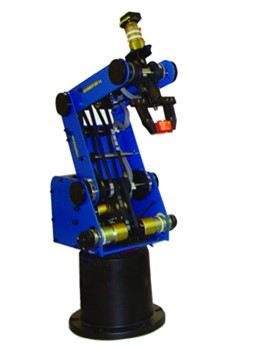
\includegraphics[scale = 0.5]{Imagenes/robot_p1.jpg}
    \caption{Figura1: Brazo SCORBOT-ER 4u }{Fuente: Profesor}
\end{figure} 
\chapter{Parte II}
\textbf{Parte II - Los estudiantes contestarán las siguientes preguntas propuestas.
}

Pág. 53 del libro

\begin{enumerate}
    \item \textbf{¿Qué se entiende por grados de libertad de un robot? Dibuje el esquema de un robot manipulador con 4 DOF.}

    R: Cada uno de los movimientos independientes que puede realizar cada articulación con respecto a la anterior.

    \begin{figure}[H]
        \centering
        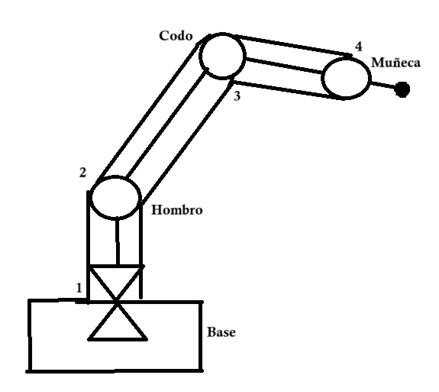
\includegraphics[scale = 0.90]{Imagenes/p1.png}
        \caption{Esquema de un robot manipulador con 4 DOF}{Fuente: Internet}
    \end{figure}

    \item \textbf{Defina con sus propias palabras las siguientes características de un robot industrial: resolución, precisión, repetibilidad, volumen de trabajo y capacidad de carga.}
    
    \begin{itemize}


        \item Precisión: Es la diferencia entre la posición alcanzada y la posición ordenada del robot. 
        \item Resolución: Es la menor variación en el posicionamiento del extremo del robot, es la precisión mínima con la que el robot puede moverse. 
        \item Repetibilidad: Se refiere a la capacidad del robot de volver a la misma posición la cantidad de veces que sea. Esta característica es muy importante porque no importa si el robot alcanzo su objetivo una vez, la idea es que lo logre las veces que sea.
        \item Volumen de trabajo: Es el alcance que tiene programado el robot para moverse y hacer sus tareas.
        \item Capacidad de carga: Es el peso máximo que un robot puede desplazar, eso incluyendo a la misma herramienta que tenga el robot. 
        
    \end{itemize}

    \item \textbf{Explique la diferencia entre los conceptos de precisión (exactitud)  y repetibilidad de un robot industrial. Emplee un dibujo para aclararlo. }
    
    R: Si un robot tiene precisión, cada vez que se le asigne una tarea, intentara hacerla lo mas completa posible y si es repetitivo entonces lograr a llegar a esa misma posición (en este caso el objetivo de la tarea u otra cosa) las veces que se le haya pedido.

    \begin{figure}[H]
        \centering
        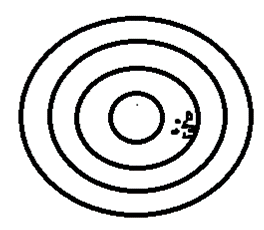
\includegraphics[scale = 0.5]{Imagenes/repeti.png}
        \caption{Repetibildiad}{Fuente:Internet}
    \end{figure}

    \begin{figure}[H]
        \centering
        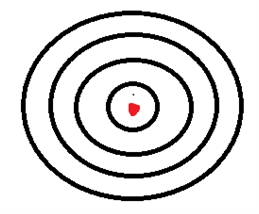
\includegraphics[scale = 0.5]{Imagenes/presicion.png}
        \caption{Precisión}{Fuente:Internet}
    \end{figure}

    \item \textbf{Enumere y describa los distintos tipos posible de articulaciones de un robot industrial.}
    
    \begin{itemize}
        \item Rótula: Permite movimiento de rotación alrededor de múltiples ejes, similar a una bola en un soporte.
        \item Prismática: permite el movimiento de traslación lineal a lo largo de un eje. 
        \item Cilíndrica: Combina una rotación alrededor de un eje y un movimiento lineal a lo largo de ese mismo eje. 
        \item Planar: Permite un movimiento de traslación en dos dimensiones, a lo largo de un plano (X, Y).
        \item Tornillo: combinación de movimientos de rotación y traslación lineal.
        \item Rotación: permite únicamente el movimiento rotacional alrededor de un eje fijo.
    \end{itemize}

    \item \textbf{Explique qué tipo de robot responde a las siguientes características: posee control de posición por topes mecánicos, su accionamiento es habitualmente neumático realizando movimientos cíclicos repetitivos de pick y place. Indique la diferencia entre un AGV y un robot móvil autónomo.}
    
    \begin{enumerate}
        \item robot secuencial. 
        \item los AGV son para carga en células robóticas y tienen una ruta predefinida y los robots móviles autónomos se desplazan de manera autónoma en su entorno.

    \end{enumerate}

    


\end{enumerate}


\chapter{Parte III}
Los estudiantes contestarán las siguientes preguntas propuestas.

\begin{enumerate}
    \item \textbf{Explique el concepto de transmisiones. Cuáles son los sistemas de transmisiones existentes. Mencione las ventajas y desventajas.}
    \item \textbf{Explique el concepto de reductores. ¿Cuáles son las características que se buscan en los reductores?}
    \item \textbf{Explique el concepto de los Accionamiento directo. ¿Cuáles son las principales ventajas de su utilización respecto a los reductores? ¿Cuál es el principal problema que plantea su utilización? ¿Explique el problema de la cinemática en los accionamientos directos?}
    \item \textbf{Explique el concepto de actuadores. ¿Cuáles son las características a considerar con los actuadores?}
    \item \textbf{Explique el concepto de sensores internos y mencione las categorías y los tipos existentes para cada categoría.}
    \item \textbf{Explique el concepto de elementos terminales. Presente una clasificación de los elementos terminales. ¿Qué tipo de accionamiento es el más empleado en los elementos terminales y por qué? ¿Cuáles son los tipos de herramientas terminales existentes?}
\end{enumerate}
\chapter{Conclusiones}
\input{4.Conclusiones/concl.tex}
\chapter{Consideraciones Finales}
\chapter{Referencias}
•	Barrientos, A. (2007). FUNDAMENTOS DE ROBOTICA (2a ED.) - ANTONIO BARRIENTOS, comprar el libro. (MCGRAW-HILL, Ed.). Retrieved from \url{http://www.casadellibro.com/libro-fundamentos-de-robotica-2-ed/9788448156367/1132459}

• Intelitek. (2023, April 3). SCORBOT ER-4U EDUCATIONAL ROBOT - Intelitek. \url{https://intelitek.com/scorbot-er-4u-educational-robot/}
\end{document}
